\section{Goal and Challenges}\label{goal}

%Goal: fare sto tool 
%challenges: performance, problemi tecnici, problemi nel testarlo dato 
%che verificare a mano le coppie è un lavoro lunghissimo. 
In my bachelor project I designed, implemented and tested a dynamic monitor component for a data flow testing tool.
The tool's purpose is the computation of the fraction of definition-use pairs covered during the execution 
of a test suite. To do so, the tool in question depends on two different components. The first one 
performs a static analysis on the program under test to compute the \textit{coverage domain}, that is, 
all the possible definition-use pairs present in the software. The second component then performs dynamic 
analysis during the execution of a test suite to check how many of the detected definition-use pairs 
were covered by the test suite.

%this is the goal
\paragraph{}
My work focused on the design, implementation and testing of the latter component: I was provided with 
a data flow analysis tool for Java called \datec \cite{Denaro}, and I was asked to implement the 
component that computes how many of the definition-use pairs identified by \datec\ were covered 
during the execution of a test suite. Figure~\ref{schema} summarizes the components and outputs of the data flow testing tool.

%these are the challenges:
%keep modularity
\paragraph{}
The main goal of this project is to complete the implementation of the data flow testing tool, still ensuring a high degree of modularity and flexibility. The coverage computation component has to interface with the output of \datec, but has to be independent and flexible to changes done to the static analysis component that, being a research tool, is frequently modified.

%acquisition of knowledge
\paragraph{}
The first challenge that I had to face was the acquisition of the theoretical knowledge about data flow
testing,  as these topics are not usually covered during Bachelor studies. The second one was the study
of the already implemented component for static analysis, as I had to interface my implementation with 
the output produced by the static analysis.

%choosing instrumentation tool
%after explanation of the tool, add modularity concern
\paragraph{}
\datec's static analysis component is not the only component my tool has to interface with, as dynamic coverage analysis requires 
a way to trace method entry and exit points as well as variable definitions and uses at runtime. To this extent, one challenge had been  
to choose a technique to perform code instrumentation from a range of candidate ones, evaluating them from their functionalities, performance,  usage complexity and compatibility with a modular design. 

Another challenge of integrating a new implementation with an existing one is the definition of a common data format. In this context, static and dynamic information are computed using different techniques and tools, using different formats and level of abstraction. Therefore, another challenge was the definition of a strategy to manipulate these formats to achieve compatibility without actually coupling the implementations. 

 \begin{figure}[h]
   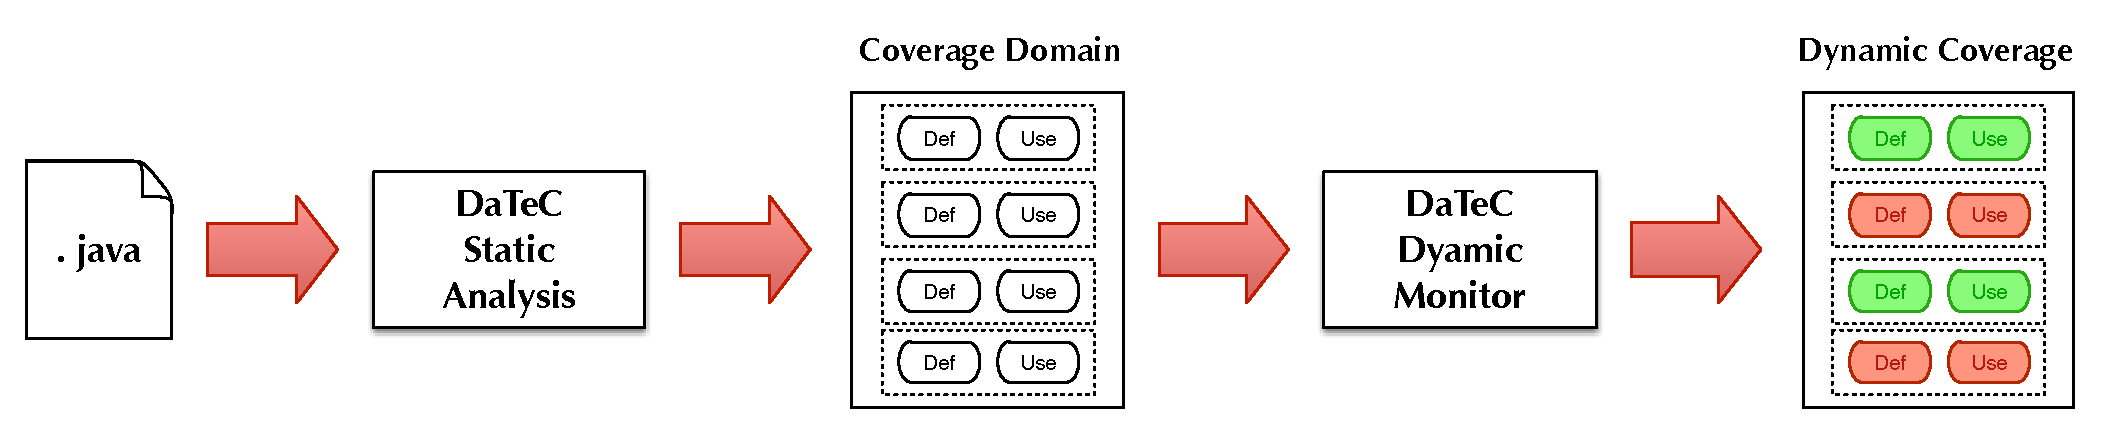
\includegraphics[width=\textwidth]{./Images/tool_highlevel.pdf}
   \caption{Exemplification of the components' role in coverage computation}
  \label{schema}
 \end{figure}

%last challenges: performance and verification
\paragraph{}
The last concern was performance and scalability, as projects could come with hundreds of test cases that produces hundreds of executions. Thus, it is important to limit the overhead of the tool to keep the execution time of big test suites within a reasonable amount of time. This is particularly challenging due to the fact that instrumentation is expensive, and that big projects have thousands of data flow elements to check.

The huge amount of analyzed data also posed a challenge in regards to the evaluation and 
verification process of the tool, as manually computing DU coverage is feasible 
only for smaller test suites, but still hard and time consuming. 